

% trial .tex file %
\documentclass[9pt]{article}  % specifies document class (article) and point size (10pt)
\usepackage{graphicx}
\usepackage{polski}
\usepackage[utf8]{inputenc}
\usepackage{sidecap}
\usepackage{wrapfig}
\usepackage{subfig}
\usepackage{amsmath}
\usepackage{float}
\usepackage{enumerate}
\usepackage{listings}
\usepackage{listings}
\usepackage{color}

\definecolor{dkgreen}{rgb}{0,0.6,0}
\definecolor{gray}{rgb}{0.5,0.5,0.5}
\definecolor{mauve}{rgb}{0.58,0,0.82}

\lstset{
  language=R,
  aboveskip=3mm,
  belowskip=3mm,
  showstringspaces=false,
  columns=flexible,
  basicstyle={\small\ttfamily},
  numbers=none,
  numberstyle=\tiny\color{gray},
  keywordstyle=\color{blue},
  commentstyle=\color{dkgreen},
  stringstyle=\color{mauve},
  breaklines=true,
  breakatwhitespace=true,
  tabsize=3
}


\begin{document}               % starts document
\author{Michał Kubica}
\title{Modele Liniowe \\ Raport nr 4}       
\maketitle                     % constructs big, fancy title

\section{Zadanie 1}            % makes a section header
  
  \subsection{a)}
    \begin{lstlisting}
    alfa = 0.05
    df = 10
    tc = qt(1-alfa/2, df)
    \end{lstlisting}  
  \subsection{b)}
    \begin{lstlisting}
    Fc = qf(1-alfa, 1, df)
    \end{lstlisting} 
  \subsection{c)}
    \begin{lstlisting}
    abs(tc^2-Fc)
    \end{lstlisting} 
    
    $8.881784 10^{-16} \approx 0$



$$CV_{(n)} = \frac{1}{n} \sum^n_{i=1} \left ( \frac{ \href{residual}{y_i - \hat{y}_i} }{ 1-h_i} \right ) ^2$$

  
\section{Zadanie 2}
  \begin{tabular}{c|c|c}
     & \textit{df} & \textit{SS} \\
    \hline
    \textit{Model} & 1 & 100 \\
    \hline
    \textit{Error} & 20 & 400 \\
  \end{tabular} 


  \subsection{a)}
  
  20+2 = 22 obseracje
  
  \subsection{b)}
  
  $s^2 = \frac{SST}{dfT} = \frac{500}{21} \approx 23.8$
  
  \subsection{c)}
  
  $H_0$ wariancje obu populacji są równe
  
  $F = \frac{MSM}{MSE} = \frac{100}{20} = 5$
  $F \sim F(1, 20)$
  $F_{kryt}(0.05,1,20) = 4.351$
  Skoro $F > F_{kryt}(0.05,1,20)$ zatem odrzucamy hipotezę zerową o niezależności.
  \subsection{d)}
  
  $R^2 = \frac{SSM}{SST} = 0.2 = 20\%$
  
  \subsection{e)}
  $|r| = \sqrt{\frac{SSM}{SST}} = \sqrt{0.2}$

\section{Zadanie 3}

  \subsection{a)}
    Dopasowany model regresji: $$Y = 0.10102 X - 3.55706 $$ , gdzie X to zmienna objaśniająca(IQ) a Y zmienna objaśniana(GPA) \newline
    $R^2 = 0.4016146$ 
    
    Przetestowano hipotezę $H_0$ : średnia ocen nie zależy od IQ, tzn $b_0 = 0$ \newline
    wartość statystyki $t = 7.142$, p-wartość $= 4.74 10^{-10}$. Wyciągnięto wniosek, że nawet przy małym poziomie istotności odrzucamy hipotezę zerową. To znaczy średnia ocen zdecydowanie zależy od poziomu inteligencji uczniów.
  


  \subsection{b)}
    Prognoza: $3.79753$ \newline
    Uzyskany 90\% przedział prognozy: $\left( 6.545114, 9.292698 \right)$



  \subsection{c)}
    \begin{figure}[H]
      \centering
      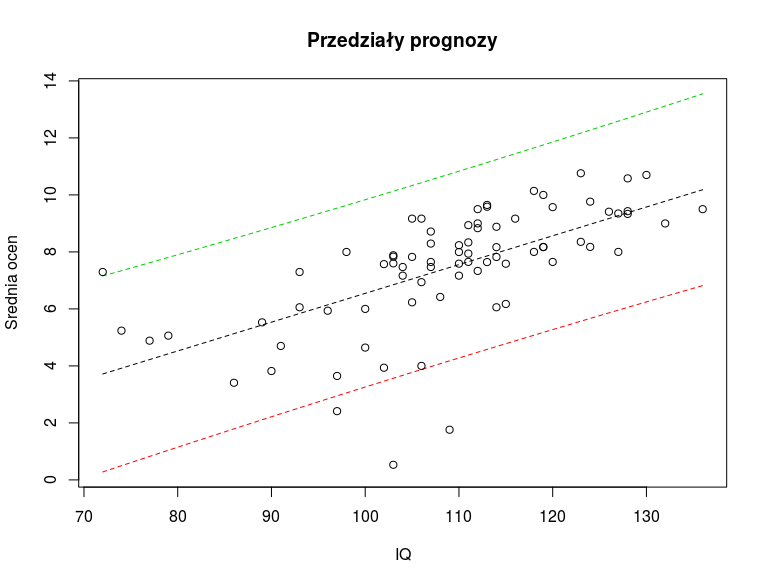
\includegraphics[width=1\textwidth]{3c.png}
      \caption {}
    \end{figure} 
    Cztery obserwacje znajdują się poza zynaczonymi przedziałami.

\section{Zadanie 4}

  \subsection{a)}
    Dopasowany model regresji: $$Y = 0.09165 X + 2.22588 $$ , gdzie X to zmienna objaśniająca(wyniki testu Piersa-Harrisa) a Y zmienna objaśniana(GPA - średnia ocen) \newline
    $R^2 = 0.2935829$ 
  
  \subsection{b)}
    Przetestowano hipotezę $H_0$ : średnia ocen nie zależy od wyników testu Piersa-Harrisa, tzn $b_0 = 0$ \newline
    wartość statystyki $t = 5.620$, p-wartość $= 3.01 10^{-7}$. Wyciągnięto wniosek, że nawet przy małym poziomie istotności odrzucamy hipotezę zerową. To znaczy średnia ocen zdecydowanie zależy od wyników testu Piersa-Harrisa uczniów.


  \subsection{c)}
    Prognoza: $4.747302$ \newline
    Uzyskany 90\% przedział prognozy: $\left( 7.72502, 10.70274 \right)$



  \subsection{d)}
    \begin{figure}[H]
      \centering
      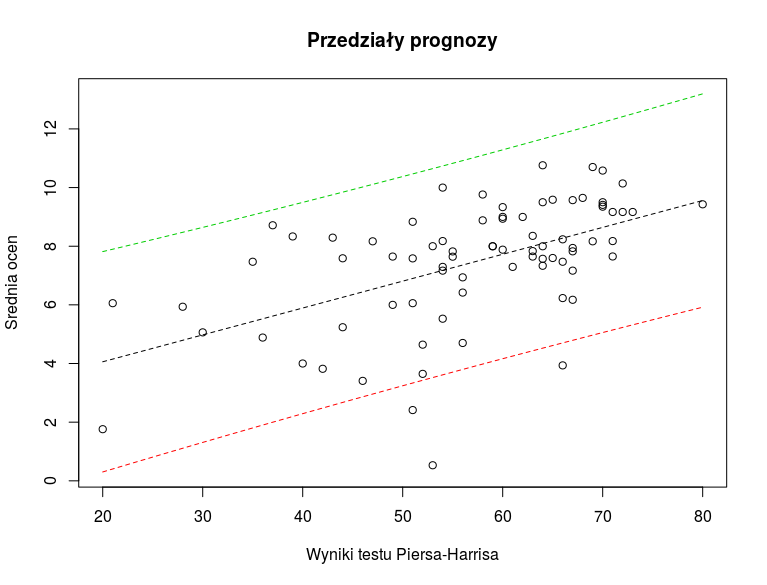
\includegraphics[width=1\textwidth]{3d.png}
      \caption {}
    \end{figure} 
    Trzy obserwacje znajdują się poza zynaczonymi przedziałami.
  
  \subsection{e)}
  
    Lepszym predyktorem średniej ocen jest poziom inteligencji.


\section{Zadanie 5}

  \subsection{a)}
  $6.883383e-15$
  \subsection{b)}
  Na poniższym wykresie nie widać żadnych zależności między zmienną objaśniającą a resztami.
      \begin{figure}[H]
      \centering
      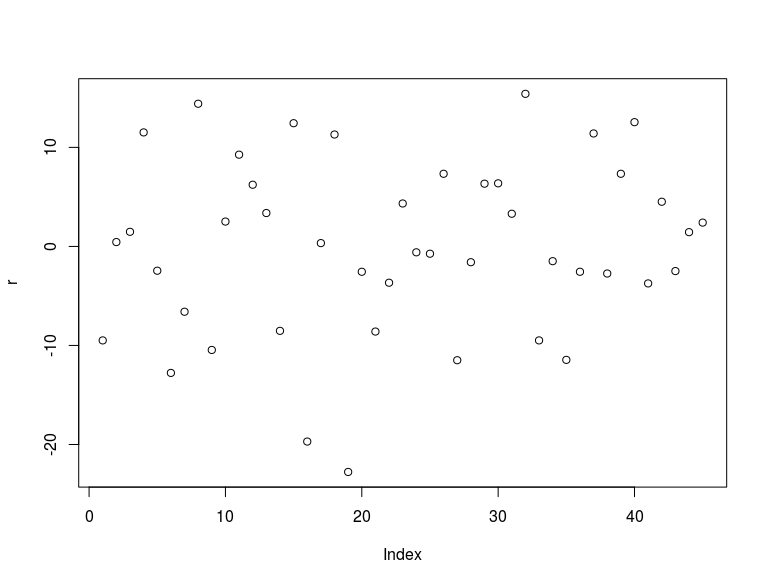
\includegraphics[width=0.7\textwidth]{5c.png}
      \caption {}
    \end{figure} 
    
  \subsection{c)}

    Na poniższym wykresie nie widać żadnych zależności między zmienną objaśniającą a resztami.
      \begin{figure}[H]
      \centering
      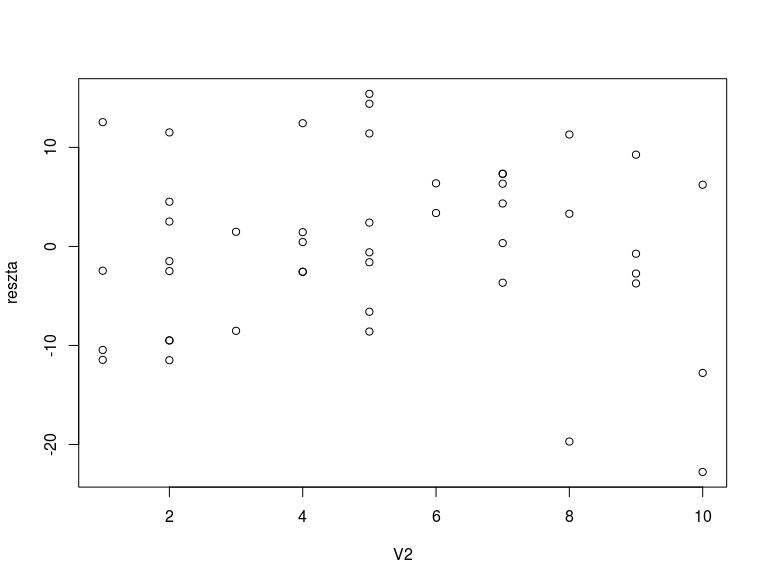
\includegraphics[width=0.7\textwidth]{5b.png}
      \caption {}
    \end{figure} 
  \subsection{d)}
    Wyznaczono histogram reszt oraz na jego tle wyrysowano wykres gęstości rozkładu normalnego. Ze względu na widoczne pdobieństwo można stwierdzić, że reszty pochodzą z rozkładu normalnego, co zgadza się z założeniami modelu regresji liniowej. 
      \begin{figure}[H]
      \centering
      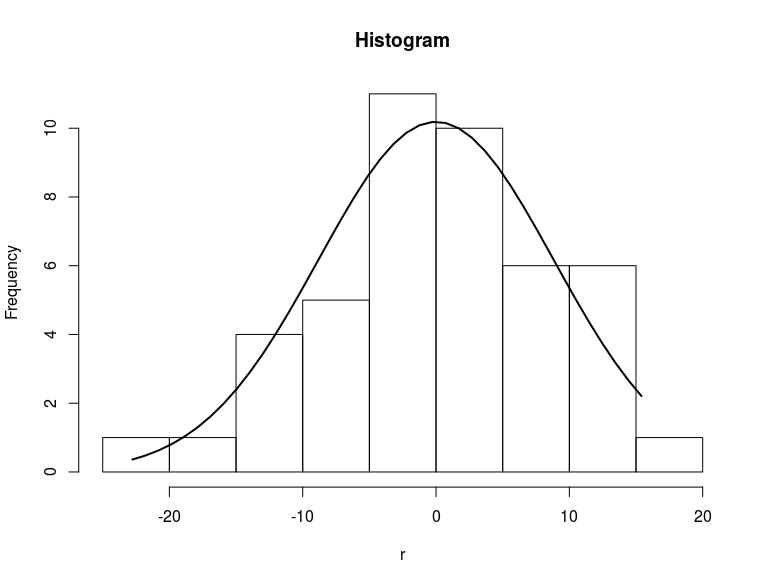
\includegraphics[width=0.7\textwidth]{5d.png}
      \caption {}
    \end{figure} 
    




\section{Zadanie 6}

  \subsection{a)}
  \begin{table}[H]
  \caption{Porównanie uzyskanych modeli}
    \begin{tabular}{c|c|c|c|c|c}
     & $b_0$ & $b_1$ & p-wartość & $R^2$ &  $\sigma^2$ \\
    \hline
    \textit{Oryginalny model} & -0.5801567 &15.035248 & $4.009032 \cdot 10^{-31}$ & 0.9574954835 & 79.45063 \\
    \hline
    \textit{Zmieniony model} & 135.9002611 & -3.058747 & 0.8480860 & 0.0008629944 & 85759.43314 \\
  \end{tabular} 
  \end{table}
  
  Na podstawie tabeli stwierdzono, że wprowadzenie do danych błędu grubego wpłynęło na wszystkie powyższe parametry. Dopasowana prosta regresji została odchylona. Estymator wariancji(miary rozrzutu danych) wzrósł bardzo mocno. P-wartość także wzrosła, do takiego poziomu, że przy testowaniu hipotezy zerowej o niezależności danych, musialibyśmy ją przyjąć. Podczas gdy w modelu oryginalnym jesteśmy pewni, że między danymi istnieje liniowa zależność. W związku z tym także drastycznie zmalał współczynnik korelacji $R^2$.
  
  \subsection{b)}
      \begin{figure}[H]
      \centering
      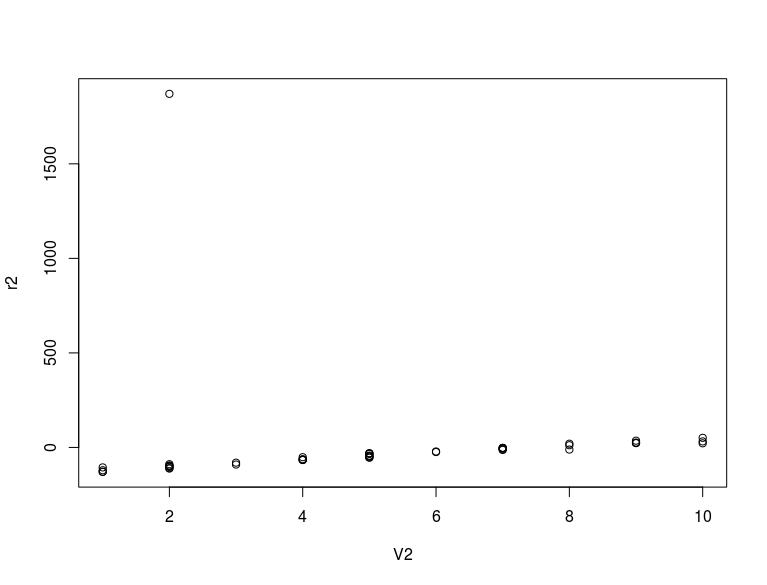
\includegraphics[width=0.7\textwidth]{6b.png}
      \caption {}
    \end{figure} 
    
  \subsection{c)}

      \begin{figure}[H]
      \centering
      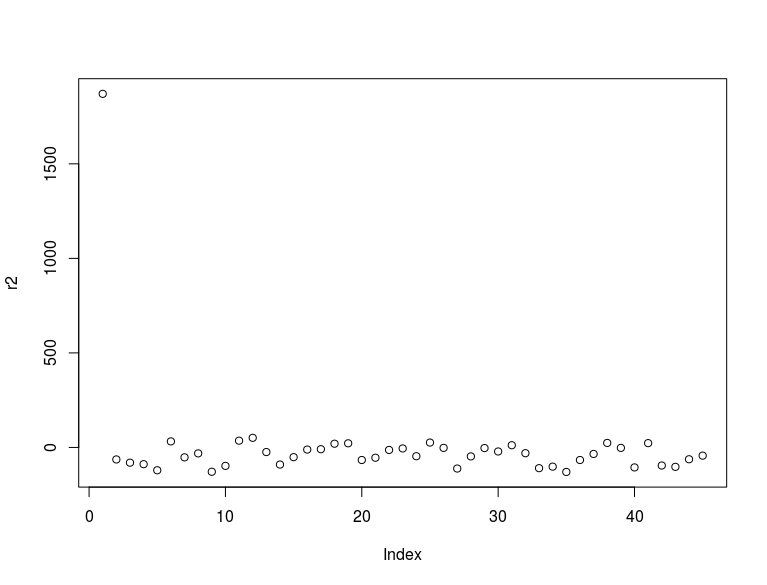
\includegraphics[width=0.7\textwidth]{6c.png}
      \caption {}
    \end{figure} 
  \subsection{d)}
    Wyznaczono histogram reszt oraz na jego tle wyrysowano wykres gęstości rozkładu normalnego.
      \begin{figure}[H]
      \centering
      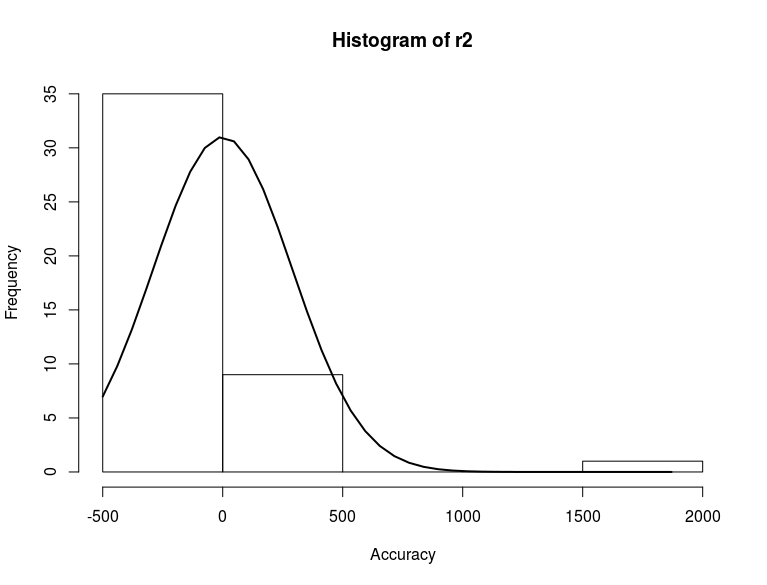
\includegraphics[width=0.7\textwidth]{6d.png}
      \caption {}
    \end{figure} 
    
        Na każdym z powyższych wykresów widać wyraźnie jedną obserwację odstającą.

\section{Zadanie 7}

  Dopasowany model regresji:
  $$ Y = -0.3240 + 2.5753$$
  $R^2$ = 0.7971 \newline
  Przetestowano następującą hipotezę: \newline
  $H_0$: stężenie roztworu nie zalezy od czasu \newline
  $H_A$: stężenie roztworu zależy od czasu \newline
  Otrzymana p-wartość: $4.61 \cdot 10^{-6}$.  \newline
  Zatem przy nawet bardzo małym poziomie istotności odrzucamy hipotezę zerową na rzecz alternatywnej. Stąd wyciągamy wniosek, że stężenie roztworu zależy od czasu. 
  


\section{Zadanie 8}

  Narysowano dane, dodano regresję oraz przedziały prognozy.
    \begin{figure}[H]
      \centering
      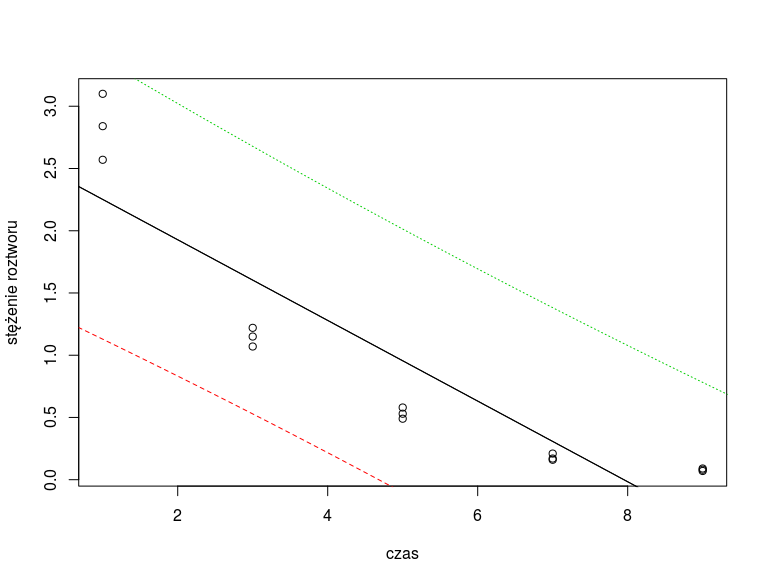
\includegraphics[width=0.7\textwidth]{8.png}
      \caption {}
    \end{figure} 
    Oraz wyznaczono współczynnik korelacji między obserwacją a prognozą stężenia roztworu: $0.9008759$


\section{Zadanie 9}
  Na wykresie z Zadania 8 można zauważyć, że możemy poszukać transformacji zmiennej objaśnianej tak, zeby lepiej dopasować prostą regresji. Do tego służy transformacja Boxa-Coxa.
    \begin{figure}[H]
      \centering
      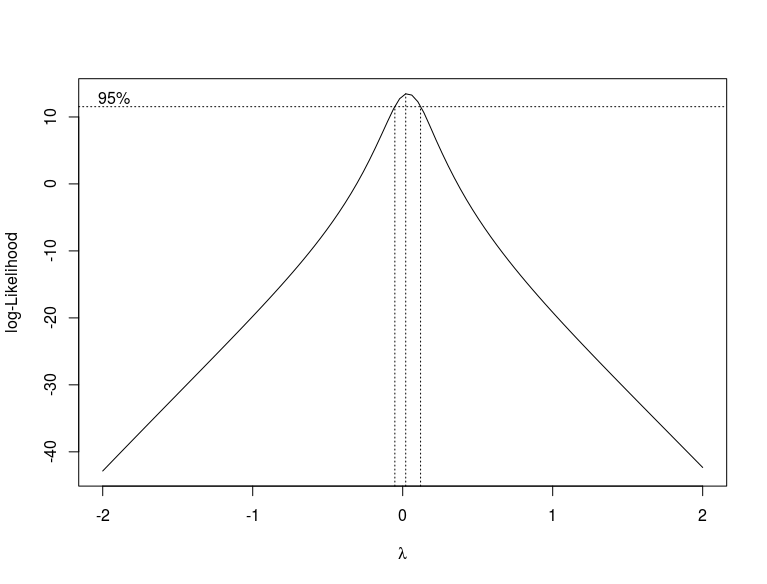
\includegraphics[width=0.7\textwidth]{9.png}
      \caption {}
    \end{figure} 
    Na podstawie wykresu zauważono, że najlepszą transformacją będzie funkcją logarytm (współczynnik $\lambda \approx$ 0)

\section{Zadanie 10}
  Przekształcono zmienną objaśnianą a następnie wykonano analizę podobną jak w zadaniu 7. \newline

  Dopasowany model regresji:
  $$ Y = -0.44993X  + 1.50792$$
  $R^2$ = 0.9924  \newline
  Przetestowano następującą hipotezę: \newline
  $H_0$: logarytm wartości stężenia roztworu nie zalezy od czasu \newline
  $H_A$: logarytm wartości stężenia roztworu zależy od czasu \newline
  Otrzymana p-wartość: $2.19 \cdot 10^{-15}$. \newline
  Zatem przy nawet bardzo małym poziomie istotności odrzucamy hipotezę zerową na rzecz alternatywnej. Stąd wyciągamy wniosek, że stężenie roztworu zależy od czasu. 
  
    Narysowano dane, dodano regresję oraz przedziały prognozy.
    \begin{figure}[H]
      \centering
      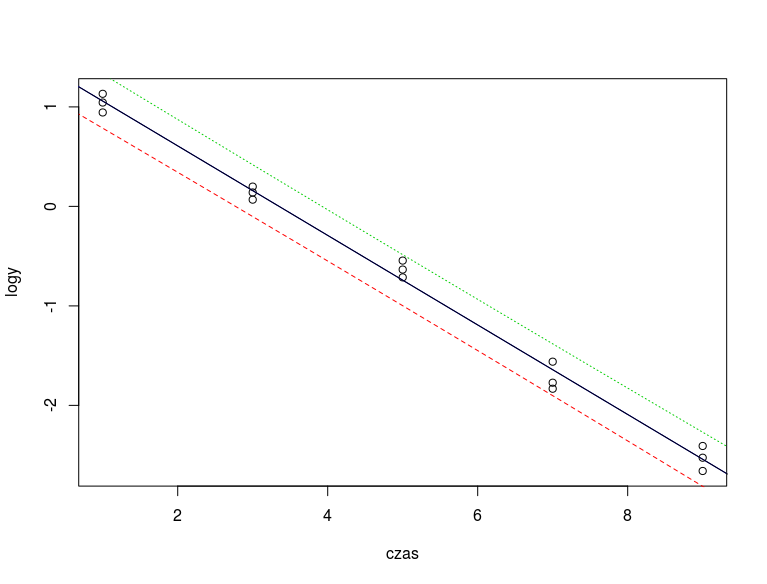
\includegraphics[width=0.7\textwidth]{10.png}
      \caption {}
    \end{figure} 
    Oraz wyznaczono współczynnik korelacji między obserwacją a prognozą logarytmem z wartości stężenia roztworu: $0.9964826$


\section{Zadanie 11}

    \begin{figure}[H]
      \centering
      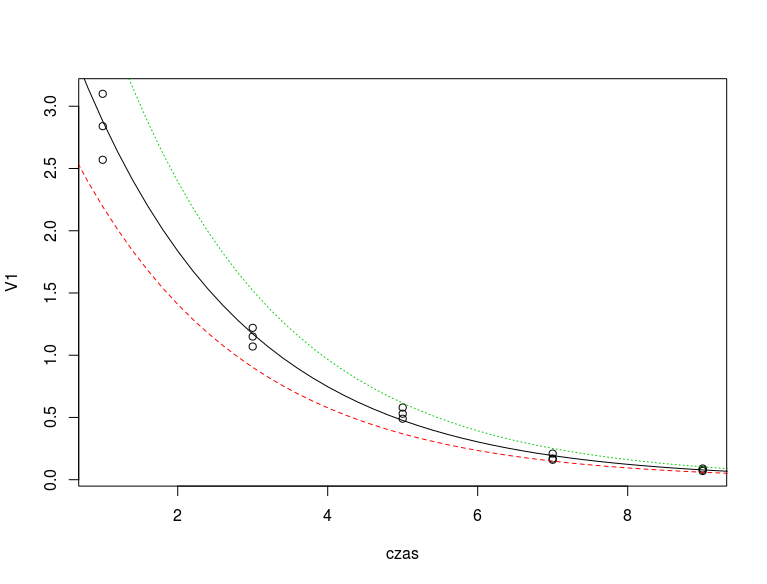
\includegraphics[width=0.7\textwidth]{11.png}
      \caption {}
    \end{figure} 
    Współczynnik korelacji między zaobserwowanym stęzeniem a prognozą z zadania 10: $0.9008759$


\section{Zadanie 12}

    Przekształcono zmienną objaśniającą ($t1 = t^{-\frac{1}{2}}$)a następnie wykonano analizę podobną jak w zadaniu 7. \newline

  Dopasowany model regresji:
  $$ Y = 4.19632X  - 1.34078 $$
  $R^2$ = 0.9871   \newline
  Przetestowano następującą hipotezę: \newline
  $H_0$: wartość stężenia roztworu nie zalezy od czasu \newline
  $H_A$: wartość stężenia roztworu zależy od czasu \newline
  Otrzymana p-wartość: $6.9 \cdot 10^{-14}$. \newline
  Zatem przy nawet bardzo małym poziomie istotności odrzucamy hipotezę zerową na rzecz alternatywnej. Stąd wyciągamy wniosek, że stężenie roztworu zależy od czasu. 


    \begin{figure}[H]
      \centering
      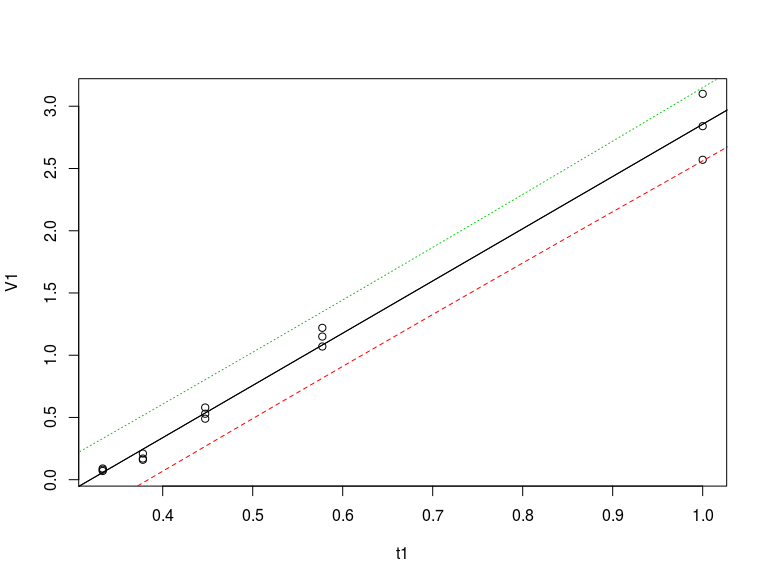
\includegraphics[width=0.7\textwidth]{12.png}
      \caption {}
    \end{figure} 
    Współczynnik korelacji: $0.9940136$
    
Porównując $R^2$ i p-wartości najlepszym modelem okazał się model z podpunktu 10. Niewiele gorszy okazał się model powyższy.
  \section{Kod R}

      \begin{lstlisting}
## ZAD 1 ##
X=runif(100)
Y=1+.3*X+rnorm(100)

summary(lm(Y~X))
abs(summary(lm(Y~X))$coefficients[2,3]^2-
summary(lm(Y~X))$fstatistic[1])

qf(0.05,1,20)

## ZAD 3 ##

# a
t=read.table(url("http://www.math.uni.wroc.pl/~mbogdan/Modele_Liniowe/Dane/table1_6.TXT"))
head(t)
attach(t)
summary(lm(V2~V3))
summary(lm(V2~V3))$r.squared
plot(V2~V3)
abline(lm(V2~V3), col='red')

# b
predict(lm(V2~V3),data.frame(V3=100),interval="prediction",level=0.9)

# c
matplot(min(t$V3):max(t$V3),predict(lm(V2~V3),data.frame(V3=min(t$V3):max(t$V3)),interval="prediction"),type="l",lty=2, main="Przedziały prognozy", xlab="IQ", ylab="Srednia ocen")
points(V3,V2)

max(t$V5)
min(t$V5)

## ZAD 4 ##

# a i b
summary(lm(V2~V5))
summary(lm(V2~V5))$r.squared

# c
predict(lm(V2~V5),data.frame(V5=60),interval="prediction",level=.9)

# d
matplot(min(t$V5):max(t$V5),predict(lm(V2~V5),data.frame(V5=min(t$V5):max(t$V5)),interval="prediction"),type="l",lty=2, main="Przedziały prognozy", xlab="Wyniki testu Piersa-Harrisa", ylab="Srednia ocen")
points(V5,V2)

# e
summary(lm(V2~V3))
summary(lm(V2~V5))


## ZAD 5 ##
t=read.table(url("http://www.math.uni.wroc.pl/~mbogdan/Modele_Liniowe/Dane/CH01PR20.txt"))
head(t)
attach(t)
plot(t[2:1])
m1=lm(V1~V2)
abline(m1,col="red")
str(summary(m1))

# a
summary(m1)$residuals
residuals(m1)
V1-m1$fitted.values
r=V1-m1$coefficients[1]-m1$coefficients[2]*V2
sum(r)
sum(summary(lm(V1~V2))$residuals)

# b
plot(V2,r, ylab="reszta")
# c
plot(r)
# d
h <- hist(r, main= "Histogram") 
xfit <- seq(min(r), max(r), length = 40) 
yfit <- dnorm(xfit, mean = mean(r), sd = sd(r)) 
yfit <- yfit * diff(h$mids[1:2]) * length(r) 

lines(xfit, yfit, col = "black", lwd = 2)

qqnorm(r)


## ZAD 6 ##

head(t)

s=t
s[1,1]=2000
heas(s)

# a
f=function(m) {v=c(m$coefficients,
summary(m)$coefficients[2,4],
summary(m)$r.squared,
summary(m)$sigma^2); names(v)=c("b0","b1","p","R2","sigma2"); v}

f(m1)

plot(s[2:1],ylim=c(-20,200))
m2=lm(s$V1~s$V2)
abline(m1,col="red")

f(m2)

View(rbind(f(m1),f(m2)))

plot(V2,residuals(m2))
identify(V2,s$V1)

# b
r2 = summary(m2)$residuals
plot(V2,r2)
plot(r2)

h <- hist(r2, xlab = "Accuracy") 
xfit <- seq(-500, max(r2), length = 40) 
yfit <- dnorm(xfit, mean = mean(r), sd = sd(r2)) 
yfit <- yfit * diff(h$mids[1:2]) * length(r2) 

lines(xfit, yfit, col = "black", lwd = 2)

qqnorm(r2)

## ZAD 7 ##

u=read.table(url("http://www.math.uni.wroc.pl/~mbogdan/Modele_Liniowe/Dane/CH03PR15.txt"))
head(u)

detach(t)

detach(u)
attach(u)
m3=lm(V1~V2)
summary(m3)

plot(V1~V2, xlab = "czas", ylab="stężenie roztworu")
abline(m3,col="black" )

## ZAD 8 ##

p=predict(m3,data.frame(V2=seq(0,10,.2)),interval="prediction")
matplot(seq(0,10,.2),p,add=TRUE,type="l")

cor(V1,predict(m3))
## ZAD 9 ##

library(MASS)
boxcox(m3)


## ZAD 10 ##
logy=log(V1)
m4=lm(logy~V2)
summary(m4)
plot(logy~V2, xlab="czas")
abline(m4,col="blue")

p=predict(m4,data.frame(V2=seq(0,10,.2)),interval="prediction")
matplot(seq(0,10,.2),p,add=TRUE,type="l")
cor(logy,predict(m4))


## ZAD 11 ##
plot(V1~V2, xlab="czas")
p=predict(m4,data.frame(V2=seq(0,10,.2)),interval="prediction")
matplot(seq(0,10,.2),exp(p),add=TRUE,type="l")
cor(V1,predict(m4))


## ZAD 12 ##
t1 = V2^(-1/2)
m5 = lm(V1~t1)
plot(V1~t1)
summary(m5)
abline(m5,col="black")

p=predict(m5,data.frame(t1=seq(0,1.2,.005)),interval="prediction")
matplot(seq(0,1.2,.005),p,add=TRUE,type="l")
cor(V1,predict(m5))



1-pchisq(2.09, 12)

chisq.test(c(1, 0, 0, 1, 0, 0, 1, 0, 1, 0, 0, 1, 0))
13*124/207



    \end{lstlisting}  



\end{document}  







